\section{IP Threat Intelligence}
\label{sec:ip-analysis}

One of the most common forms of \ti\ are feeds of IP addresses considered malicious,
suspicious, or otherwise untrustworthy. This type of threat intelligence dates back
at least to the early spam and intrusion detection blacklists, many of which are
still active today such as SpamhausSBL~\cite{SpamhausSBL}, CBL~\cite{CBL} and
SORBS~\cite{SORBS}. Here, I apply the metrics described above to quantify the
differences between \numipfeeds\ different IP address \ti\ feeds.
%The overview of the these feeds is summarized in Table~\ref{tab:volume-overview-1}.


\subsection{Feed Categorization}
IP address \ti\ feeds have different meanings, and, therefore, purposes. To
meaningfully compare feeds to each other, I first group feeds into
\emph{categories} of feeds whose indicators have the same intended meaning.
Unfortunately, there is no standard or widely accepted taxonomy of IP \ti\ feeds.
To group feeds into semantic categories, I use metadata associated with the
feed as well as descriptions of the feed provided by the producer, as described below.

\emphpar{Metadata} Some feeds provide category information with each indicator as
metadata. More specifically, all of the {Paid Aggregator} feeds, {\feedalienvault}
and {\feedetiprep} include this category metadata. In this case, I use its pre-assigned
category in the feed. Facebook ThreatExchange feeds do not include category
information in the metadata, but instead provide a descriptive phrase with each indicator.
I then derive its category based on the description.

\emphpar{Feed description} For feeds without metadata, I rely on online descriptions
of each feed, where available, to determine its semantic category. For example, the
website of feed {\feednothink}~\cite{Nothink} describes that the feed reports brute-force
login attempts on its corresponding honeypot, which indicates the feed belongs to
brute-force category.

I grouped the IP feeds into categories derived from the information
above. In this work, I analyze six of the most prominent categories:
%, listed below.
%
\begin{categorylist}\small
\item[Scan] Hosts doing port or vulnerability scans.
\item[Brute-force] Hosts making brute force login attempts.
\item[Malware] Malware C\&C and distribution servers.
\item[Exploit] Hosts trying to remotely exploit vulnerabilities.
\item[Botnet] Compromised hosts belonging to a botnet.
\item[Spam] Hosts that sent spam or should not originate email.
\end{categorylist}
%
Table~\ref{tab:volume-overview-1} lists the feeds, grouped by category, used in the
rest of this section. The symbols \snapfeedsym\ and \deltafeedsym\ before the feed
name indicate whether the feed is a snapshot feed or an event feed, respectively
(see Section~\ref{sec:feed-structure}).
All data was collected during my measurement period,
\veryemph{December 1st, 2017} to \veryemph{July 20th, 2018}. Note that a few
feeds, like {\feedetiprep}, appear in multiple categories. In these feeds, indicators
are associated with different categories via attached metadata. I split these feeds
into multiple virtual feeds each containing indicators belonging to the same category.

\subsection{Volume}
\label{sec:ip-volume}

%\noteby{KL}{Change this to Size and Rate.}
Volume is one of the oldest and simplest \ti\ metrics representing how informative
each data source is. Table~\ref{tab:volume-overview-1} and Table~\ref{tab:volume-overview-2} shows the total number of unique IP addresses
collected from each feed during the measurement period, under column \emph{Volume}. A \snapfeedsym\ denotes a \textit{snapshot feed}
and \deltafeedsym\ indicates an \textit{event feed} (Section~\ref{sec:feed-structure}).
\colname{Volume} is the total number of IPs collected during our measurement period.
\colname{Exclusive} is the exclusive contribution of each feed (Section~\ref{sec:ip-unique}).
\colname{Avg. Rate} is the number of average daily new IPs added in the feed (Section~\ref{sec:ip-accuracy}), and
\colname{Avg. Size} is the average working set size of each feed (Section~\ref{sec:ip-volume}).
Feeds are listed in order of decreasing volume, grouped by category.
The numbers we show are after the removal of invalid entries identified
by the sources themselves. Column \emph{Avg. Rate} shows the average number of
new IPs we received per day, and \emph{Avg. Size} lists the average daily
working set size of each feed, that is, the average size of the snapshot.

\finding\ Feeds vary dramatically in volume. Within every category, big feeds can contain
orders of magnitude more data than small feeds. For example, in the scan category, we saw
over 361,004 unique IP addresses in \feeddshield\ but only 1,572 unique addresses
in \feedTSAnalyst\ in the same time period. Clearly, volume is a major differentiator
for feeds. %In Section~\ref{sec:ip-overlap} and~\ref{sec:ip-unique}, we will examine which
%feeds duplicate each other and which feeds contribute unique indicators.

%\newcolumntype{H}{>{\setbox0=\hbox\bgroup}c<{\egroup}@{}}

\begin{table}[t!]
\centering
\caption{IP \ti\ feeds used in the study part I}
\label{tab:volume-overview-1}
\small
 \begin{tabular}{l@{}r r r r}
 \toprule
 \colname{Feed} & \colname{Volume} & \colname{Exclusive} & \colname{Avg. Rate} &  \colname{Avg. Size} \\ %& \colname{Unrt} \\
  \midrule
  \textbf{Scan Feeds} \\
  %\cline{1-1}

\snapfeedsym\  {\feedTSAlienVault}\footnote{This feed is aggregated by \emph{PA} from Alienvault OTX,
                                            the {\feedalienvault} is the public reputation feed we collected
                                            from AlienVault directly. They are different feeds.}

                                     & 425,967 	& 48.6\% 	& 1,359  & 128,821 \\
\deltafeedsym\ {\feeddshield}        & 361,004 	& 31.1\% 	& 1,556  & 69,526 \\
\snapfeedsym\  {\feedTSramnode}      & 258,719 	& 62.0\% 	& 870    & 78,974 \\
\deltafeedsym\ {\feedpacketmail}     & 246,920 	& 48.6\% 	& 942    & 29,751 \\
\snapfeedsym\  {\feedetiprep}        & 204,491 	& 75.6\% 	& 1,362  & 8,756 \\
\snapfeedsym\  {\feedTSLabScan}      & 169,078 	& 63.1\% 	& 869 	 & 9,775 \\
\snapfeedsym\  {\feedTSSnort}        & 19,085 	& 96.3\% 	& 56     & 4,000 \\
\deltafeedsym\ {\feedFBBasecamp}     & 6,066 	& 71.3\% 	& 24     & 693 \\
\snapfeedsym\  {\feedTSAnalyst}      & 1,572 	& 34.5\% 	& 6.3 	 & 462 \\


  %\midrule
  \textbf{Botnet Feeds} \\
  %\cline{1-1}
\snapfeedsym\  {\feedTSAnalyst}     & 180,034 	& 99.0\% 	& 697 	    & 54,800 \\
\snapfeedsym\  {\feedTSCI}          & 103,281 	& 97.1\% 	& 332 	    & 30,388 \\
\snapfeedsym\  {\feedetiprep}       & 77,600 	& 99.9\% 	& 567 	    & 4,278 \\
\snapfeedsym\  {\feedTSBotscout}    & 23,805 	& 93.8\% 	& 81 	    & 7,180 \\
\snapfeedsym\  {\feedTSVoIP}        & 10,712 	& 88.0\% 	& 40 	    & 3,633 \\
\snapfeedsym\  {\feedTSCompr}       & 7,679 	& 87.0\% 	& 21 	    & 2,392 \\
\snapfeedsym\  {\feedTSBots}        & 4,179 	& 80.7\% 	& 16 	    & 1,160 \\
\snapfeedsym\  {\feedTSHoneypot}    & 2,600 	& 86.5\% 	& 8.5 	    & 812 \\


  %\midrule
  \textbf{Brute-force Feeds} \\
  %\cline{1-1}
\deltafeedsym\  {\feedbadipssh}     & 542,167 	& 84.1\% 	& 2,379 	& 86,677 \\
\deltafeedsym\  {\feedbadipbot}     & 91,553 	& 70.8\% 	& 559 	    & 17,577 \\
\snapfeedsym\   {\feedetiprep}      & 89,671 	& 52.8\% 	& 483 	    & 3,705 \\
\snapfeedsym\   {\feedTSBrute}      & 41,394 	& 92.1\% 	& 138 	    & 14,540 \\
\deltafeedsym\  {\feedusername}     & 37,198 	& 54.2\% 	& 179 	    & 3662.8 \\
\deltafeedsym\  {\feeddisco}        & 31,115 	& 43.6\% 	& 40 	    & 1,224 \\
\deltafeedsym\  {\feedFBZendesk}    & 22,398 	& 77.3\% 	& 74 	    & 2,086 \\
\deltafeedsym\  {\feednothink}      & 20,325 	& 62.7\% 	& 224 	    & 12,577 \\
\deltafeedsym\  {\feeddangerrule}   & 10,142 	& 4.88\% 	& 37	    & 1,102 \\

  %\midrule
  \textbf{Malware Feeds} \\
  %\cline{1-1}
\snapfeedsym\  {\feedetiprep} 	     & 234,470 	& 99.1\% 	& 1,113 	& 22,569 \\
\deltafeedsym\ {\feedFBAdmin} 	     & 30,728 	& 99.9\% 	& 129 	    & 3,873 \\
\snapfeedsym\  {\feedfeodo} 	     & 1,440 	& 47.7\% 	& 1.3 	    & 1,159 \\
\snapfeedsym\  {\feedTSLabMalware}   & 1,184 	& 84.6\% 	& 3.5 	    & 366 \\
\deltafeedsym\ {\feedmalcode} 	     & 865 	    & 61.0\% 	& 2.9 	    & 86.6 \\
\snapfeedsym\  {\feedTSBambenek}     & 785 	    & 92.1\% 	& 3.4 	    & 97.9 \\
\snapfeedsym\  {\feedTSSSL} 	     & 676 	    & 53.9\% 	& 2.9 	    & 84.0 \\
\snapfeedsym\  {\feedTSAnalyst}	     & 492 	    & 79.8\% 	& 2.1 	    & 149 \\
\snapfeedsym\  {\feedTSAbusech}      & 256 	    & 7.03\% 	& 1.6 	    & 117 \\
\snapfeedsym\  {\feedTSMalTraffic}   & 251 	    & 60.5\% 	& 0.9 	    & 72 \\
\snapfeedsym\  {\feedzeus}           & 185 	    & 49.1\% 	& 0.5 	    & 101 \\
\bottomrule
\end{tabular}
\end{table}


\begin{table}[t!]
\centering
\caption{IP \ti\ feeds used in the study part II}
\label{tab:volume-overview-2}
\small
 \begin{tabular}{l@{}r r r r}
 \toprule
 \colname{Feed} & \colname{Volume} & \colname{Exclusive} & \colname{Avg. Rate} &  \colname{Avg. Size} \\ %& \colname{Unrt} \\
  \midrule
  %\midrule
  \textbf{Exploit Feeds} \\

\deltafeedsym\  {\feedbadiphttp}    & 305,020 	& 97.6\% 	& 1,592 	& 22,644 \\
\deltafeedsym\  {\feedbadipftp}     & 285,329 	& 97.5\% 	& 1,313 	& 27,601 \\
\deltafeedsym\  {\feedbadipdns}     & 46,813 	& 99.3\% 	& 231 	& 4,758 \\
\deltafeedsym\  {\feedbadiprfi}     & 3,642 	& 91.4\% 	& 16 	& 104 \\
\deltafeedsym\  {\feedbadipsql}     & 737 	    & 79.5\% 	& 4.4 	& 99.2 \\

 \textbf{Spam Feeds} \\
  %\cline{1-1}
\snapfeedsym\  {\feedetiprep}       & 543,583 	& 99.9\% 	& 3,280 	& 6,551 \\
\deltafeedsym\ {\feedbadippostfix}  & 328,258 	& 90.5\% 	& 842 	    & 27,951 \\
\deltafeedsym\ {\feedbadipspam}     & 302,105 	& 89.3\% 	& 1,454 	& 30,197 \\
\snapfeedsym\  {\feedTSBotscout}    & 14,514 	& 89.3\% 	& 49 	& 4,390 \\
\snapfeedsym\  {\feedalienvault}    & 11,292 	& 96.6\% 	& 48 	& 1,328 \\

\bottomrule
\end{tabular}
\end{table}

%\footnotetext{}



Average daily rate represents the amount of new indicators collected from a feed each day.
Some feeds may have large volume but low daily rates, like {\feedfeodo} in the malware
category. This means most indicators we get from that feed are old data present in the feed before our
measurement started. On the other hand, the average rate of a feed could be
greater than the volume would suggest, like {\feednothink} in the brute-force category.
This is due to the fact that indicators can be added and removed multiple times in a
feed. In general, IP indicators tend to be added in a feed only once: 37 among \numipfeeds\
IP feeds have over 80\% of their indicators appearing only once, and 30 of them have this rate over 90\%.
One reason is that some snapshot feeds maintain a valid period for each indicator, as
we found in all \emph{PA} feeds where the expiration date of each indicator is explicitly
recorded. When the same indicator is discovered again by a feed before its expiration time,
the feed will just extend its expiration date, so this occurrence will not be captured
if we simply subtract the old data from the newly collected data to derive what is added on a day.
For event feeds and snapshot feeds in \emph{PA} where we can precisely track every occurrence
of each indicator, we further examed data occurrence frequency and still found that the vast
majority of IPs in feeds only occurred once---an observation that relates to the dynamics
of cyber threats themselves.

\feednothink, as we mentioned above, is a notable exception. It has over 64\% of its
indicators appearing 7 times in our data set. After investigating, we
found that this feed posts all its previous data at the end of every month, behavior very likely
due to the feed provider instead of the underlying threats.
% {\feedusername}, {\feedbadipftp}, {\feedbadipdns} and {\feedbadipsql}
% all have a large percent of IPs appeared twice, and we found
% that all 4 feeds reported a abnormally large amount of same IPs on 2018 July 1st and July 13th.
% We will discuss more about this in Section~\ref{sec:ip-accuracy}.

The working set size defines the daily average amount of indicators users need to store in their
system to use a feed (the storage cost of using a feed). The average
working set size is largely decided by the valid period length
of the indicators, controlled either
by the feed (snapshot feeds) or the user (event feeds). The longer the valid period is,
the larger the working set will be. Different snapshoot feeds have different choices for this
valid period: {\feedTSAlienVault} in the scan category sets a 90-day valid period for
every indicator added to the feed, while {\feedTSAbusech} uses a 30-day period. Although we do not
know the data expiration mechanism used by snapshot feeds other than \emph{PA} feeds, as
there is no related information recorded, we can still roughly estimate this by checking the
\emph{durations} of their indicators---the time between an indicator being added and being removed.
Four {\feedetiprep} feeds have more than 85\% of durations shorter than 10 days, while the one in
the malware category has more than 40\% that span longer than 20 days. {\feedfeodo} has over 99\% of
its indicators valid for our entire measurement period, while over 70\% of durations in the
{\feedzeus} are less than 6 days. We did not observe a clear pattern regarding how each snapshot
feed handles the expiration of indicators.

%The column \emph{Occurred} presents the number of unique IPs added in a \ti\ source after our
%measurement period started. We differentiate \emph{Volume} and \emph{Occurred} since IP
%indicators are time sensitive: They are added, removed and could be added again in a feed over
%time. When we pull data from a snapshot feed on a day, some IPs are actually added
%on previous days and are still kept by the feed. \emph{Occurred} only captures the IPs that
%are newly added after the measurement period started, while \emph{Volume} includes legacy data in
%a feed when we collect indicators on the first day of our analysis. At a high level,
%\emph{Volume} represents the number of IPs that a feed \emph{considers} as malicious during
%a period of time, and \emph{Occurred} represents the number of newly discovered indicators by the
%feed during that time.

%For delta feeds, we calculated their \emph{Volume} by tracking the expiration dates of the
%indicators we collected before (The expiration dates are provided in the metadata) and included
%the indicators whose expiration dates are after January 1st, 2016.

\subsection{Differential Contribution and Intersection}
\label{sec:ip-overlap}

%It is often useful to know whether a potential new feed contributes any new indicators relative to what a \ti\ consumer has already.
The differential contribution metric measures the number of indicators in one feed that are not in another. Equivalently, we can consider the intersection of two feeds, which is the number of elements in one feed that are present in the other, normalized by the size of the first: $|A\cap B|/|A|$. Figure~\ref{fig:overall_heatmap} shows the intersection relationship of all feeds in the study. Each cell in the matrix represents the number of elements in both feeds, normalized by the size of the feed spanning the rows on the table. That is, $A$, in the expression above, ranges over rows, and $B$ over columns of the matrix. Darker (more saturated) colors indicate greater intersection. Comparisons of feeds within a category are shaded red and comparisons of feeds between different categories are shaded blue. Note that the matrix is asymmetric, because, in general, $|A\cap B|/|A| \neq |A\cap B|/|B|$. Elements of the matrix are in the same order as in Table~\ref{tab:volume-overview-1}.

\begin{figure}
\centering
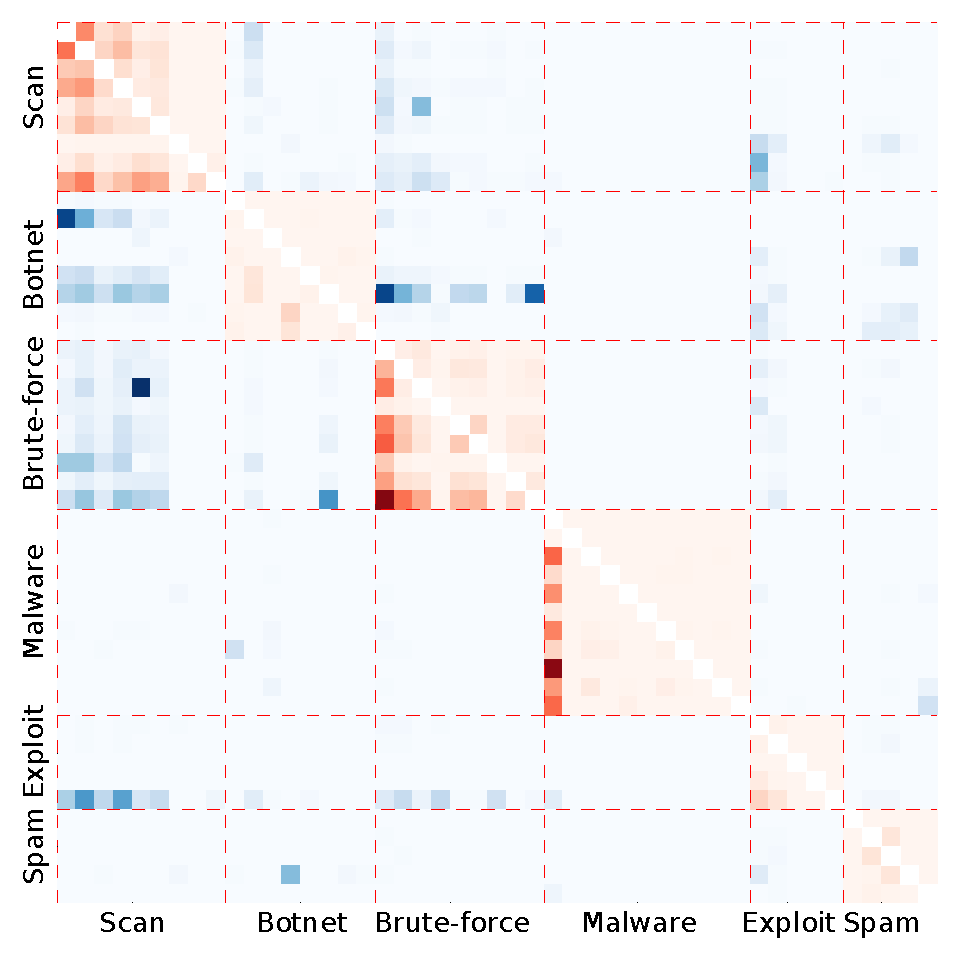
\includegraphics[width=0.475\textwidth]{images/overall_heatmap.pdf}
\caption{Feed intersection for all IP feeds. Each row/column represents a feed, shown in the same order as Table~\ref{tab:volume-overview-1}. Darker (more saturated) colors indicate greater intersection.}
\label{fig:overall_heatmap}
\end{figure}

%\begin{figure}
%\centering
%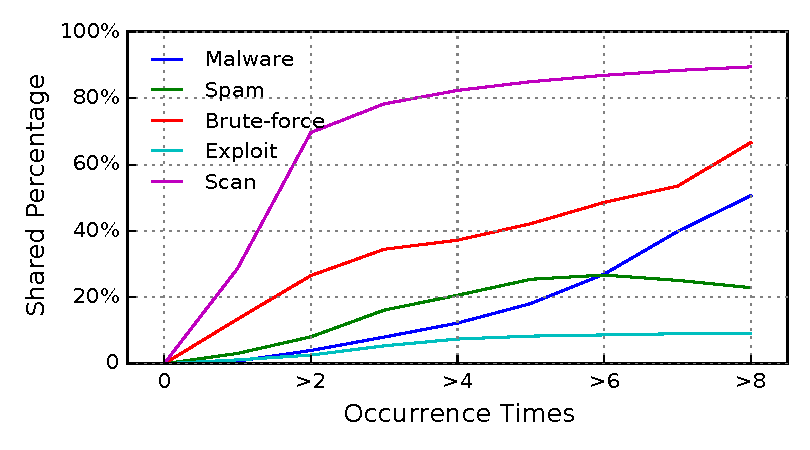
\includegraphics[width=0.4\textwidth]{images/occur_vs_overlap.pdf}
%\caption{Relation between indicators' occurrence frequency and the percentage of being shared. Each point on a line means: For the %indicators that had occurred >\emph{x} times in a feed(\textbf{X} axis), how much percent of them are shared among at least two feeds within its category(\textbf{Y} axis).}
%\label{fig:occur_vs_overlap}
%\end{figure}

\finding\ Feeds in scan and brute-force categories have higher pairwise intersections: Half of the pairwise intersection rates in two categories are greater than 5\%. The scan category has 29 out of 72 pairs (excluding self comparisons) with an intersection rate larger than 10\%, and the same case occurred in 19 out of 72 pairs in the brute-force category.

On the other side, feeds in the botnet, exploit, malware and spam category do not share much data between each other: all 4 categories have more than three-quarters of pairwise intersection rates less than 1\%. A few big feeds in these categories can share a significant amount of data with some small feeds in the same category---a characteristic that appears as a dark vertical line within its category in Figure~\ref{fig:overall_heatmap}. \feedetiprep\ in the malware category, for example, shares over 30\% of 6 other malware feeds. But the intersections among the vast majority of feeds in these 4 categories are low. This finding is consistent with prior work~\cite{metcalf2015blacklist,thomas2016abuse}, but we provide a more comprehensive view regarding different categories.

Figure~\ref{fig:overall_heatmap} also shows the relation between feeds across different categories. We can clearly see a relation between scan and brute-force feeds: multiple scan feeds have non-trivial intersection with feeds in the brute-force category. In fact, 23.1\% of all 760,263 brute-force IPs we collected are also included by scan feeds in our dataset. There are also three botnet feeds---\feedTSCI, \feedTSVoIP\ and \feedTSCompr---that have over 10\% of its data shared with multiple feeds in the scan category.

%\noteby{KL}{Cut this paragraph and accompanying figure.}
%One interesting question is: Are indicators that occurred multiple times in a feed more likely to be shared between feeds? We check this question by calculating how much percent of indicators, that had occurred more than \emph{x} times in a feed, are shared between at least two feeds within each category. The result is shown in Figure~\ref{fig:occur_vs_overlap}. Botnet category is excluded from the Figure since the percentages are too low to argue about the trend. We can see that there is a strong positive correlation between the occurrence frequency and the percentage being shared, across different categories. This aligns with the intuition that a persistent attacker is more likely being observed by mulitple \ti\ sources.

\subsection{Exclusive Contribution}
\label{sec:ip-unique}

Exclusive contribution represents the number of indicators in a feed that are in no other feeds. I calculate each feed's exclusive contribution among all the feeds in the same category, emphasizing their uniqueness regarding the scope of data they claim to report. Each feed's exclusive contribution is presented in Table~\ref{tab:volume-overview-1} in column \emph{Exclusive}, calculated based on its volume.

\finding\ As I already observed in Section~\ref{sec:ip-overlap}, botnet, exploit and spam feeds have relatively low pairwise intersections. Consequently, the feeds in these four categories have high exclusive contribution rates in general: the median exclusive contribution rates of these four categories are 90.9\%, 97.5\% and 90.5\%, respectively. The malware category has a low median exclusive rate, since multiple small feeds have non-trivial intersection with the largest feed {\feedetiprep}, but the two largest feeds in malware both have a exclusive rate over 99\%. Scan and brute-force feeds have more intersection within its category, and their exclusive rates are lower: 62.0\% median rate in scan and 62.7\% in brute-force, and the top two largest feeds in both categories have an exclusive rate below 85\%.

If one assumes a process where a feed is more likely to have popular elements, then smaller feeds would be subsumed by larger feeds. Yet, for some small feeds like {\feedmalcode} in the malware and {\feedTSHoneypot} in the botnet categories, even though they are several orders of magnitude smaller than the largest feeds in their categories, a significant proportion of their indicators is still unique to the feed. When I aggregate the data in each category, 73\% of all scan feed indicators are unique to a single feed and 88\% of brute force feed indicators are unique to one feed. For other categories, over 97\% of elements in the category are unique to a single feed. This result agrees with previous work that most data in threat intelligence feeds is unique~\cite{metcalf2015blacklist,thomas2016abuse}.
\subsection{Latency}
\label{sec:ip-timing}

% Data Occurrence analysis
Feed latency measures how quickly a feed reports new threat indicators. The
sooner a feed can report potential threats, the more valuable it is for
consumers. The absolute latency of an indicator in a feed is the time from
the beginning of the corresponding event until when the indicator shows up in
the feed. However, it is difficult to know the actual time when an event begins
from the threat intelligence data. Instead, we measure the \textit{relative
latency}, which is the delay of an indicator in one feed to be the time between
its appearance in that feed and the first seen among all the feeds.

\begin{figure}[t!]
\centering
\subfloat[Latency distribution in scan feeds]{
	\label{fig:scan_firstseen}
	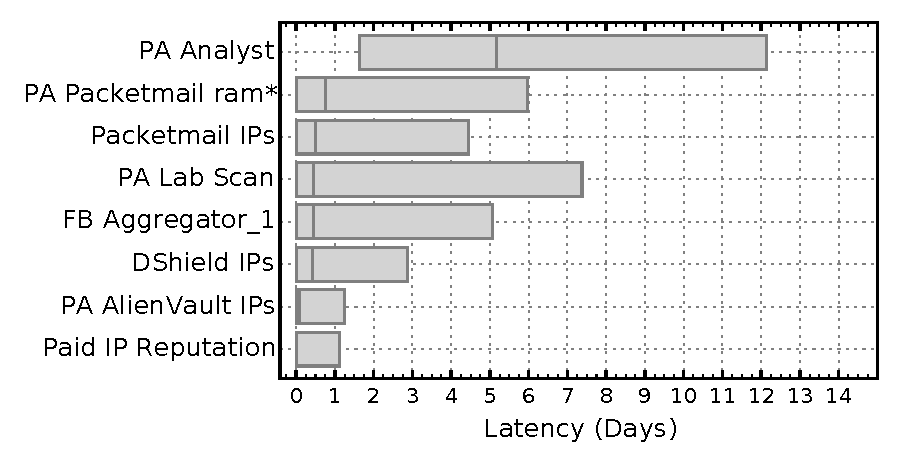
\includegraphics[width=0.8\textwidth]{data_character/images/scan_latency_new.pdf}}

\subfloat[Latency distribution in brute-force feeds]{
	\label{fig:brute_firstseen}
	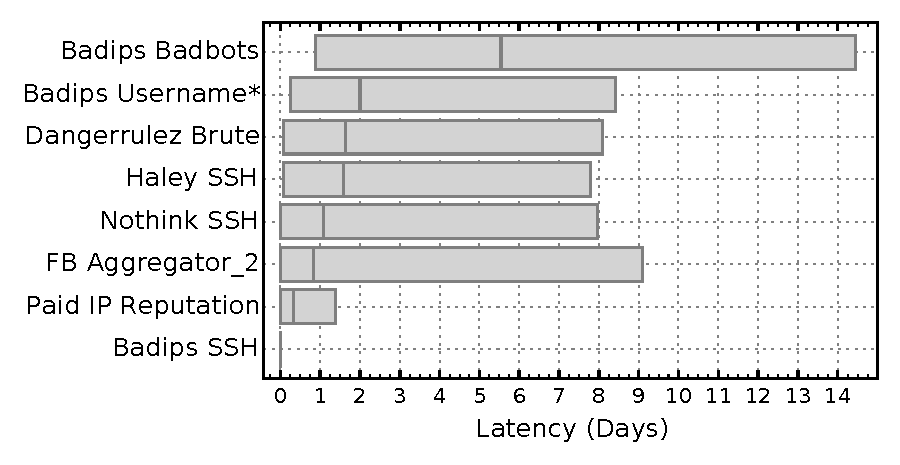
\includegraphics[width=0.8\textwidth]{data_character/images/brute_latency_new.pdf}}

\caption{Distribution of indicators' latency in scan and brute-force feeds.}
\label{fig:firstseen}
\end{figure}


Relative latency can only be calculated for
indicators that occur in at least two feeds. As discussed in
Section~\ref{sec:ip-unique}, the number of common indicators in the botnet, malware, exploit and spam feeds is very low (fewer than 3\% of elements occur in more than one feed). Relative latency calculated for these feeds is less meaningful. For this analysis, therefore, we focus on scan and brute-force feeds.

Another issue is the time sensitivity of IP threats. An event that originated from
an IP address, like scanning activity or a brute-force attack, will not last
forever. If one scan feed reports an IP address today and another feed reports
the same IP three months later, it would make little sense to consider them as one
scanning event and label the second occurrence as being three months late.
Unfortunately, there is no easy way we can clearly distinguish events from each
other. Here we use a one-month window to restrict an event, assuming that the same
attack from one source will not last for more than 30 days; although arbitrary, it provides a reasonably conservative threshold, and experimenting with other thresholds produced similar overall results. More specifically, we calculate relative latency by tracking the
first occurrence of IPs in all feeds in a category, then recording the latency of the
following occurrences while excluding ones that occur after 30 days. By just
using the first appearance of each IP as the base, we avoid the uncertainty caused by
multiple occurrence of indicators and different valid periods used among feeds.

%We also used other time windows for the latency calculation and the results are very similar.

Figures~\ref{fig:scan_firstseen} and~\ref{fig:brute_firstseen} show the relative
latency distribution among feeds in the scan and brute-force categories, in hours. Each box shows the latency distribution of shared IPs in the feed calculated in hours
from 25 percentile to 75 percentile, with the middle line indicating the median.
(``Badips Username*'' here is the abbreviation for feed name Badips
Username Notfound; ``PA Packetmail Ram*'' for PA Packetmail Ramnode)
We focus on just those feeds that have
over 10\% of their data shared with others to ensure the analysis can represent the latency
distribution of the overall feed. There is one feed in each category ({\feedTSSnort}
in scan and {\feedTSBrute} in brute-force) that is excluded from the figure.

\finding\
From the distribution boxes we can see that {\feedetiprep} in scan and {\feedbadipssh}
in brute-force are the fastest feeds in their category, as they have the lowest median
and 75th percentile latencies. On the other hand, {\feedTSAnalyst} in scan and
{\feedbadipbot} in brute-force are the slowest feeds. Figure~\ref{fig:scan_firstseen}
shows that all scan feeds except one have their 25th percentile latency equal to 0, indicating
these feeds, across different sizes, all reported a significant portion of their shared
data first. A similar case also happens in the brute-force category.

%This means that feeds can scan feeds, no matter fast or slow,

One may reasonably ask whether large feeds report data sooner than small feeds.
The result shows that this is not always the case. {\feedFBBasecamp} is the second smallest
feed in our scan category, yet it is no slower than several other feeds which have over 10 times of its daily rate.
{\feedbadipbot}, on the other hand, has the second largest rate in brute-force
category, but it is slower than all the other feeds in the brute-force category. Feeds that are small in volume can still report a lot of their data first.

% This shows that when choosing a feed, we cannot assume its latency by just looking at its volume.

Another factor that could affect latency is whether feeds copy data from each other. For example, 93\% of {\feeddangerrule} also appears in {\feedbadipssh}. If this is the case, we expect {\feeddangerrule} will be faster than {\feedbadipssh} on
reporting their shared data. However, we compared the relative latency between just two feeds and found {\feedbadipssh} reported 88\% of their shared indicators first.
We further conducted this pairwise latency comparison between all feeds in scan, brute-force
and malware (since {\feedetiprep} shares non-trivial amount of data with a
few small feeds in the malware category), and did not see a clear latency advantage between
any two feeds. Note that this observation does \emph{not} prove there is no data
copying, since the shared data between two feeds might partially come from copying and partially from the feeds' own data collection. Furthermore, our latency analysis is at a one-hour granularity.
% We did not find the evidence in latency to prove that there is indeed data copying.

\subsection{Accuracy}
\label{sec:ip-accuracy}
\newcolumntype{H}{>{\setbox0=\hbox\bgroup}c<{\egroup}@{}}

\begin{table}[t!]
\centering
\caption{IP \ti\ feeds accuracy overview. \colname{Unrt} is fraction of unroutable addresses in each feed (Section~\ref{sec:ip-accuracy}).
\colname{Alexa Top} is the number of IPs intersected with top Alexa domain IP addresses, and
\colname{CDNs} is the number of IPs intersected with top CDN provider IP addresses.}
\label{tab:accuracy-overview-1}
\scriptsize
 \begin{tabular}{l r r r r}
 \toprule
 \colname{Feed} & \colname{Added} & \colname{Unrt} & \colname{Alexa} &  \colname{CDNs} \\ %& \colname{Unrt} \\
  \midrule
  \textbf{Scan Feeds} \\
  %\cline{1-1}
{\feedTSAlienVault}  & 313,175 	& 0.0\% 	& 1  & 0 \\
{\feeddshield}       & 339,805 	& 0.03\% 	& 68 & 62\\
{\feedTSramnode}     & 200,568 	& <0.01\% 	& 0  & 0 \\
{\feedpacketmail}    & 211,081 	& 0.0\% 	& 0  & 0 \\
{\feedetiprep}       & 200,915 	& 1.65\% 	& 6  & 21\\
{\feedTSLabScan}     & 169,037 	& <0.01\% 	& 0  & 0 \\
{\feedTSSnort}       & 12,957 	& 0.42\% 	& 1  & 0 \\
{\feedFBBasecamp}    & 5,601 	& 0.0\% 	& 0  & 0 \\
{\feedTSAnalyst}     & 1,451 	& 0.41\% 	& 0  & 0 \\


  %\midrule
  \textbf{Botnet Feeds} \\
  %\cline{1-1}
{\feedTSAnalyst}     & 180,034 	& <0.01\% 	& 0  & 0 \\
{\feedTSCI}          & 76,125 	& <0.01\% 	& 0  & 0 \\
{\feedetiprep}       & 73,710 	& 1.66\% 	& 6  & 74\\
{\feedTSBotscout}    & 18,638 	& 0.09\% 	& 1  & 0 \\
{\feedTSVoIP}        & 9,290   	& 0.32\% 	& 0  & 0 \\
{\feedTSCompr}       & 4,883 	    & 0.0\% 	& 0  & 0 \\
{\feedTSBots}        & 3,594 	    & 0.0\% 	& 0  & 0 \\
{\feedTSHoneypot}    & 1,947 	    & 0.0\% 	& 0  & 0 \\


  %\midrule
  \textbf{Brute-force Feeds} \\
  %\cline{1-1}
{\feedbadipssh}     & 456,605 	& 0.19\% 	& 217  & 1\\
{\feedbadipbot}     & 91,553 	& 1.04\% 	& 46   & 1,251\\
{\feedetiprep}      & 87,524 	& 0.03\% 	& 0  & 10\\
{\feedTSBrute}      & 31,555 	& 0.0\% 	& 0  & 0\\
{\feedusername}     & 37,198 	& 0.53\% 	& 4  & 0\\
{\feeddisco}        & 8,784 	& 0.03\% 	& 0  & 0\\
{\feedFBZendesk}    & 17,779 	& 0.0\% 	& 0  & 0\\
{\feednothink}      & 20,325 	& 1.51\% 	& 2  & 0\\
{\feeddangerrule}   & 8,247 	& 0.0\% 	& 0  & 0\\


  %\midrule
  \textbf{Malware Feeds} \\
  %\cline{1-1}

{\feedetiprep}       & 217,073 	& 0.13\% 	& 291  & 3,489\\
{\feedFBAdmin}       & 29,840 	& 2.14\% 	& 2    & 0\\
{\feedfeodo}         & 296 	& 0.0\% 	& 0   & 0\\
{\feedTSLabMalware}  & 806 	& 2.85\% 	& 0   & 0\\
{\feedmalcode}       & 668 	& 0.0\% 	& 8   & 11\\
{\feedTSBambenek}    & 777 	& 9.13\% 	& 0   & 0\\
{\feedTSSSL}         & 674 	& 0.0\% 	& 0   & 0\\
{\feedTSAnalyst}     & 486 	& 0.0\% 	& 0   & 0\\
{\feedTSAbusech}     & 256 	& 3.12\% 	& 0   & 0\\
{\feedTSMalTraffic}  & 193 	& 0.51\% 	& 0   & 0\\
{\feedzeus}          & 67 	& 0.0\% 	& 1   & 0\\

  %\midrule
  \textbf{Exploit Feeds} \\
{\feedbadiphttp}    & 305,020 	& 0.67\% 	& 16  & 2,590\\
{\feedbadipftp}     & 285,329 	& 1.33\% 	& 14  & 2\\
{\feedbadipdns}     & 46,813 	& 0.50\% 	& 119 & 244 \\
{\feedbadiprfi}     & 3,642 	& 2.22\% 	& 0   & 0\\
{\feedbadipsql}     & 737 	& 1.89\% 	& 0   & 1\\

  \textbf{Spam Feeds} \\
  %\cline{1-1}
{\feedetiprep}      & 543,546 	& 78.7\% 	& 1	& 0 \\
{\feedbadipspam}    & 302,105 	& 0.02\% 	& 19	& 0 \\
{\feedbadippostfix} & 193,674 	& 1.29\% 	& 18	& 1 \\
{\feedTSBotscout}   & 11,358 	& 0.06\% 	& 0  	& 0 \\
{\feedalienvault}   & 10,414 	& 0.07\% 	& 63	& 1,040 \\

\bottomrule
\end{tabular}
\end{table}

%\footnotetext{}


Accuracy measures the rate of false positives in a feed. A false
positive is an indicator that data is labeled with a category to which
it does not belong.  For example, an IP address found in a scan feed
that has not conducted any Internet scanning is one such false
positive.  As well, even if a given IP is in fact associated with
malicious activity, if it is not unambiguously actionable (e.g.,
Google's DNS at 8.8.8.8 is used by malicious and benign software
alike) then for many use cases it must also be treated as a false
positive.  False positives are problematic for a variety of reasons,
but particularly because they can have adverse operational
consequences.  For example, one might reasonably desire to block all
new network connections to and from IP addresses reported as hosting
malicious activity (indeed, this use is one of the promises of threat
intelligence). False positives in such feeds, though, could lead to
blocking legitimate connections as well.  Thus, the degree of accuracy
for a feed may preclude certain use cases.

Unfortunately, determining which IPs belong in a feed and which do not
can be extremely challenging. In fact, at any reasonable scale, I am
unaware of any method for unambiguously and comprehensively
establishing ``ground truth'' on this matter.  Instead, in this
section I report on a proxy for accuracy that provides a
conservative assessment of this question.  To wit, I assemble a
\emph{whitelist} of IP addresses that either should not reasonably be
included in a feed, or that, if included, would cause significant
disruption. The presence of such IPs in a feed are
clearly false positives and thus define an upper bound on a feed's
accuracy.  I populate my list from three sources: unroutable IPs,
IPs associated with top Alexa domains, and IPs of major content
distribution networks (CDNs). The detail result for the accuracy analysis 
is presented in Table~\ref{tab:accuracy-overview-1} and 
Table~\ref{tab:accuracy-overview-2}.
\colname{Unrt} is fraction of unroutable addresses in each feed
(Section~\ref{sec:ip-accuracy}).
\colname{Alexa Top} is the number of IPs intersected with top Alexa domain 
IP addresses, and \colname{CDNs} is the number of IPs intersected with 
top CDN provider IP addresses. I will explain more about each column in below.

\noindent\textbf{Unroutable IPs.} Unroutable IPs are IP addresses that
were not BGP-routable \emph{when they first appeared} in a feed, as
established by contemporaneous data in the RouteViews
service~\cite{Routeview}. While such IPs could have appeared in the
source address field of a packet (i.e., due to address spoofing), it
would not be possible to complete a TCP handshake. Feeds that imply
that such an interaction took place should not include such IPs. For
example, feeds in the Brute-force category imply that the IPs they
contain were involved in brute-force login attempts, but this could
not have taken place if the IPs are not routable. While including
unroutable addresses in a feed is not, in itself, a problem, their
inclusion suggests a quality control issue with the feed, casting
shade on the validity of other indicators in the feed.

To allow for some delays in the feed, I check if an IP was routable
at any time in the seven days prior to its first appearance in a feed,
and if it had, I do not count it as
unroutable. Table~\ref{tab:accuracy-overview-1}, column \textit{Unrt},
shows the fraction of IP indicators that were not routable at any time
in the seven days prior to appearing in the feed. This analysis is
only conducted for the IPs that are added after my measurement
started. The number of such IPs is shown in column \textit{Added}, and
the unroutable fraction shown in \textit{Unrt} is with respect to this
number.

\noindent\textbf{Alexa.} Blocking access to popular Internet sites or
triggering alarms any time such sites are accessed would be disruptive
to an enterprise. For my analysis, I periodically collected the
Alexa top 25 thousand domains (3--4 times a month) over the course of
the measurement period~\cite{alexa}. To address the challenge that
such lists can have significant churn~\cite{scheitle2018long}, we
restrict my whitelist to hold the \emph{intersection} of all these
top 25K lists (i.e., domains that were in the top 25K every time we
polled Alexa over the 8-month measurement period), which left us with
12,009 domains. I then queried DNS for the A records, NS
records and MX records of each domain, and collected the corresponding
IP addresses. In total, I collected 42,436 IP addresses associated
with these domains. I compute the intersection of these IPs
with \ti\ feeds and show the results in column \textit{Alexa} in
Table~\ref{tab:accuracy-overview-1}.


\noindent\textbf{CDNs.} CDN providers serve hundreds of thousands of
sites. Although these CDN services can (and are) abused to conduct
malicious activities~\cite{cdnabuse}, their IP addresses are not
actionable.  Because these are fundamentally shared services,
blocking such IP addresses will also disrupt access to benign
sites served by these IPs.  I collected the IP ranges used by 5
popular CDN providers: AWS CloudFron~\cite{cloudfront},
Cloudflare~\cite{cloudflare}, Fastly~\cite{fastly},
EdgeCast~\cite{edgecast} and MaxCDN~\cite{maxcdn}. I then check how
many IPs in \ti\ feeds fall into these ranges. Column \textit{CDNs} in
Table~\ref{tab:accuracy-overview-1} shows the result.

\finding\ Among the \numipfeeds\ feeds in the table, 33 feeds have at
least one unroutable IP, and for 13 of them, over 1\% of the addresses
they contain are unrouteable. Notably, the {\feedetiprep} feed in the
spam category has an unroutable rate over 78\%.  Although it is not
documented, a likely explanation is that this feed may include unroutable
IPs intentionally, as this is a known practice among certain spam
feeds. For example, the Spamhaus DROP List~\cite{Spamhaus} includes IP
address ranges known to be owned or operated by malicious actors,
whether currently advertised or not. Thus, for feeds that explicitly
do include unroutable IPs, their presence in the feeds should not
necessarily be interpreted as a problem with quality control.

I further checked feeds for the presence of any ``reserved IPs''
which, as documented in RFC 8190, are not globally routable (e.g., private
address ranges, test networks, loopback and multicast).  Indeed,
12 feeds reported at least one reserved IP, including four of the
{\feedetiprep} feeds (excepting the spam category), six of the Badips
feeds, and the {\feedFBAdmin} and {\feeddshield} feeds. Worse, the
{\feedetiprep} feeds together reported over 100 reserved IPs. Since
such addresses should never appear on a public network,
reporting such IPs indicates that a feed provider fails to
incorporate some basic sanity checks on its data.

There are 21 feeds that include IPs from top Alexa domains, as shown
in column \textit{Alexa} in Table~\ref{tab:accuracy-overview-1}. Among
these IPs there are 533 A records, 333 IPs of MX records and 63 IPs of
NS records.  The overlapped IPs include multiple instances from
notable domains. For example, the IP addresses of www.github.com are
included by {\feedmalcode}.  {\feedetiprep} in the malware category
contains the IP address for www.dropbox.com.  {\feedalienvault}
contains the MX record of groupon.com, and {\feedbadipssh} also
contains the IP addresses of popular websites such as www.bing.com.

Most of the feeds I evaluated do not contain IPs in CDN ranges, yet
there are a few (including multiple {\feedetiprep} feeds, Badips feeds
and {\feedalienvault}) that have significant intersection with CDN
IPs. {\feedalienvault} and Badips feeds primarily intersect with
%IPs from
Cloudflare CDN, while most of the overlap in the {\feedetiprep} malware
category overlaps with AWS CloudFront.

Overall, the rate of false positives in a feed is not strongly
correlated with its volume.  Moreover, certain classes of false
positives (e.g., the presence of Top Alex IPs or CDN IPs) seem to
be byproducts of how distinct feeds are collected (e.g., Badips
feeds tend to contain such IPs, irrespective of volume).
Unsurprisingly, I also could find not correlation between a feed's
latency and its accuracy.
\subsection{Coverage}
\label{sec:completeness}

The coverage metric provides a quantitative measure of how well a
feed captures the intended threat. A feed with perfect
coverage would include all indicators that belong in a category.
Unfortunately, as discussed above, there is no systematic way for
evaluating the exact accuracy or coverage of a feed since it is unrealistic
to obtain ground truth of all threat activities on the Internet.

However, there are some large-scale threat activities that are
well-collected and well-studied. One example is Internet
scanning. Researchers have long been using ``Internet telescopes'' to
observe and measure network scanning
activities~\cite{benson2015leveraging, durumeric2014internet,
  pang2004characteristics}.  With a large telescope and well-defined
scan filtering logic, one can obtain a comprehensive view of global
scanning activities on the Internet.

To this end, we collected three months of traffic (from January 1st to
March 31st 2018) using the UCSD network telescope~\cite{telescope},
which monitors a largely quiescent /8 network comprising over 16
million IP addresses.  We then used the default parameters of the Bro
IDS~\cite{BroNetwork} to identify likely scanning traffic, namely
flows in which the same source IP address is used to contact 25 unique
destination IP addresses on the same destination port/protocol within
5 minutes. Given the large number of addressed being monitored, any
indiscriminate scanner observed by \ti\ feeds will likely also be seen
in our data.  Indeed, by intersecting against this telescope data we
are able to partially quantify the coverage of each \ti\ scanning feed.


%(u'TS Alien Vault OTX Malicious IPs', 'scan') 0.966922702159 0.0045119148556
%(u'dshield-ips', 'scan') 0.951590802754 0.00826350821018
%(u'TS Packetmail iprep ramnode', 'scan') 0.933286248198 0.00306798601481
%(u'packetmail-ip', 'scan') 0.87635529608 0.00365935255666
%(u'et-ip-reputation', 'scan') 0.627009603999 0.00230524603455
%(u'TS Anomali Labs MHN', 'scan') 0.855805914736 0.0032333616247
%(u'TS Snort IP BlockList', 'scan') 0.0862598022503 1.2237504915e-05
%(u'FB Basecamp Streetcred', 'scan') 0.153300600109 1.3591853285e-05
%(u'TS Analyst', 'scan') 0.523206751055 1.19956569917e-05

The scanners we collected from the telescope consist of 20,674,149 IP addresses.
The total number of IPs in all the scan feeds during this period is
425,286, which covers only 1.7\% (363,799 shared IPs) of all the telescope scan IPs.
On the other hand, telescope scanners intersect with 85\% of all IPs in scan feeds.
When looking at each feed, {\feedTSAlienVault}, {\feeddshield}
{\feedpacketmail}, {\feedTSLabScan} and {\feedTSramnode} all have over 85\% of their
data intersected with telescope scanners; the other four, though, have less than 65\%
of their data shared (and the rate for {\feedTSSnort} is only 8\%).


To further understand how well each scan feed detects scanning
activities, we measure how different sizes of scanners in the
telescope are covered by each feed. Here, \emph{scanner size} means how
many IPs a scanner has scanned in the telescope within a
day. Figure~\ref{fig:caida_coverage_cdf} shows the coverage rate of
each feed over different sizes of scanners, ranging from 1,000 to
1 million. \textbf{Y} axis is the proportion of scanners of a given size or 
larger that are covered by each feed. (There are 7,212,218 scanners from the 
telescope whose sizes
are over 1K, 271,888 that are over 100K and 17,579 are over 1 million.)


\begin{figure}
\centering
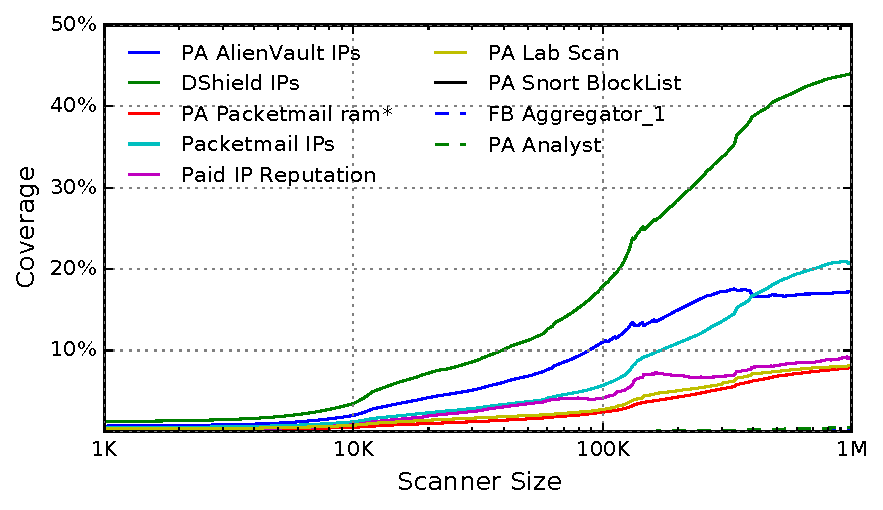
\includegraphics[width=0.8\textwidth]{data_character/images/caida_coverage_cdf.pdf}
\caption{The coverage of each feed on different sizes of scanners.}
\label{fig:caida_coverage_cdf}
\end{figure}

\finding\
The union of all the scan IPs in the feeds covers less than
2\% of the scanners collected by the telescope. Even if we only look
at the scanners with sizes larger than 10,000, the overall coverage is still
around 10\%, suggesting the coverage capability of scan feeds
is very limited. The graph shows that, as the scanner size increases, the coverage of
each feed over the datasets also increases, and large feeds cover more percent
of telescope scanners than small feeds. This trend aligns with the intuition that
scan feeds tend to capture more extensive scanners.

It is surprising that the small scan feeds in our collection have a smaller percentage of their
IPs shared with telescope scanners. This contradicts the idea that small feeds
would contain a larger percentage of extensive scanners (that would most likely also be observed by the telescope).

%Using another metric, the volume of scanners in the
%telescope is over 20 times larger than that of the scan feeds, yet the
%telescope scanners only cover 25.9\% of all of the scanning feeds'
%data. The overall volume of scanning activities is so extensive that
%even a /8 telescope will miss many of them, particularly if scanners
%are selective in targets (avoiding or focusing on certain IP ranges)
%or rate limits (falling below scanner labeling thresholds). The
%coverage curve based on scanner sizes showed that scan feeds are
%better at capturing large scanners, which is intuitive, but that a
%larger feed does not necessarily mean better coverage.


%\begin{table}
%\small
%\caption{Intersection between scan feeds and telescope scanners.
%\textit{Volume} contains the total amount of IPs in each feed from
%Jan. 2016 to July 2016. \textit{Intersection} is the proportion
%of each feed's IPs that overlap with the telescope data.}
%\centering
% \resizebox{0.7\linewidth}{!}{
%\begin{tabular}{l r r }
%\toprule
%Feed & Volume & Intersection \\
%\midrule
%{PA Snort BlockList}     & 312,533   & 18.2\% \\
%{\feedetiprep}           & 293,484   & 22.1\% \\
%{\feedpacketmail}        & 50,723    & 83.6\% \\
%{PA Packetmail ramnode}  & 11,452    & 76.1\% \\
%{\feedalienvault}        & 8,695     & 35.1\% \\
%{PA Malicious IPs}       & 7,960     & 63.3\% \\
%{PA Packetmail CARISIT}  & 5,955     & 71.5\%\\
%{PA SANS Top IPs}        & 3,087     & 77.4\%\\
%{PA Analyst}             & 444       & 52.0\%\\
%{PA Shockpot IPs}        & 156       & 50.0\%\\
%{PA SANS IPs}            & 129       & 63.6\%\\
%{FB Aggregator}          & 103       & 37.9\%\\
%\midrule
%Total & 675,243 & 25.9\%\\
%\bottomrule
%\end{tabular}
%}
%\label{tab:caida_ip_overlap}
%\end{table}

